\chapter{嵌入式实现}

\section{GPU嵌入式开发平台简介}
GPU 是图像处理单元(Graphics Process Unit)的缩写,它最先由 NVIDIA 公 司提出,是一种专门用于图像和图形处理的并行处理器。GPU 在图像处理、数据 分析等方面有着得天独厚的优势,近些年来得到了广泛的发展和应用。如今的 GPU 在计算吞吐量及内存带宽上已经远远超过 CPU,特别是对于并行计算以及浮点运 算,GPU 的性能要远远高于 CPU,这使得 GPU 成为当今世界上处理并行数据最 有效的处理器。

\subsection{Jetson TK1 开发平台简介}
2014 年 5 月 NIVDIA 公司发布了全球首款高性能 GPU 嵌入式开发平台 Jetson TK1。它是一款专门为开发人员设计的高性能、低功耗的 GPU 嵌入式开发套件, 可用于开发机器人、汽车自动驾驶、无人机等应用和系统。
Jetson TK1 平台上包含一颗拥有 192 个 CUDA 核心的 Terga K1 移动处理器, 该处理器采用了 NIVDIA 公司最新推出的 GPU 架构——Kepler 架构。同时该处理 器上集成了一颗四核 ARM® Cortex-A15 CPU,最高主频为 2.3GHz。Terga K1 拥有 326 gflops 的浮点运算能力,其运算能力比类似的嵌入式平台多 3 倍以上。相对于 强大的处理性能,该处理器的功耗却极低。
Jetson TK1 开发平台除了搭载业界最强悍的 Terga K1 移动处理器之外,另含 2GB 运行内存和 16GB 的扩展存储空间,同时该平台拥有麦克风输入、USB 3.0、HDMI 1.4、千兆以太网口、SD/MMC、SATA、miniPCIe、RS232 串行端口、Micro
USB 等丰富的 I/O 端口。图 \ref{fig:tk1} 展示了 Jetson TK1 开发平台的硬件架构。
\begin{figure}
	\centering
	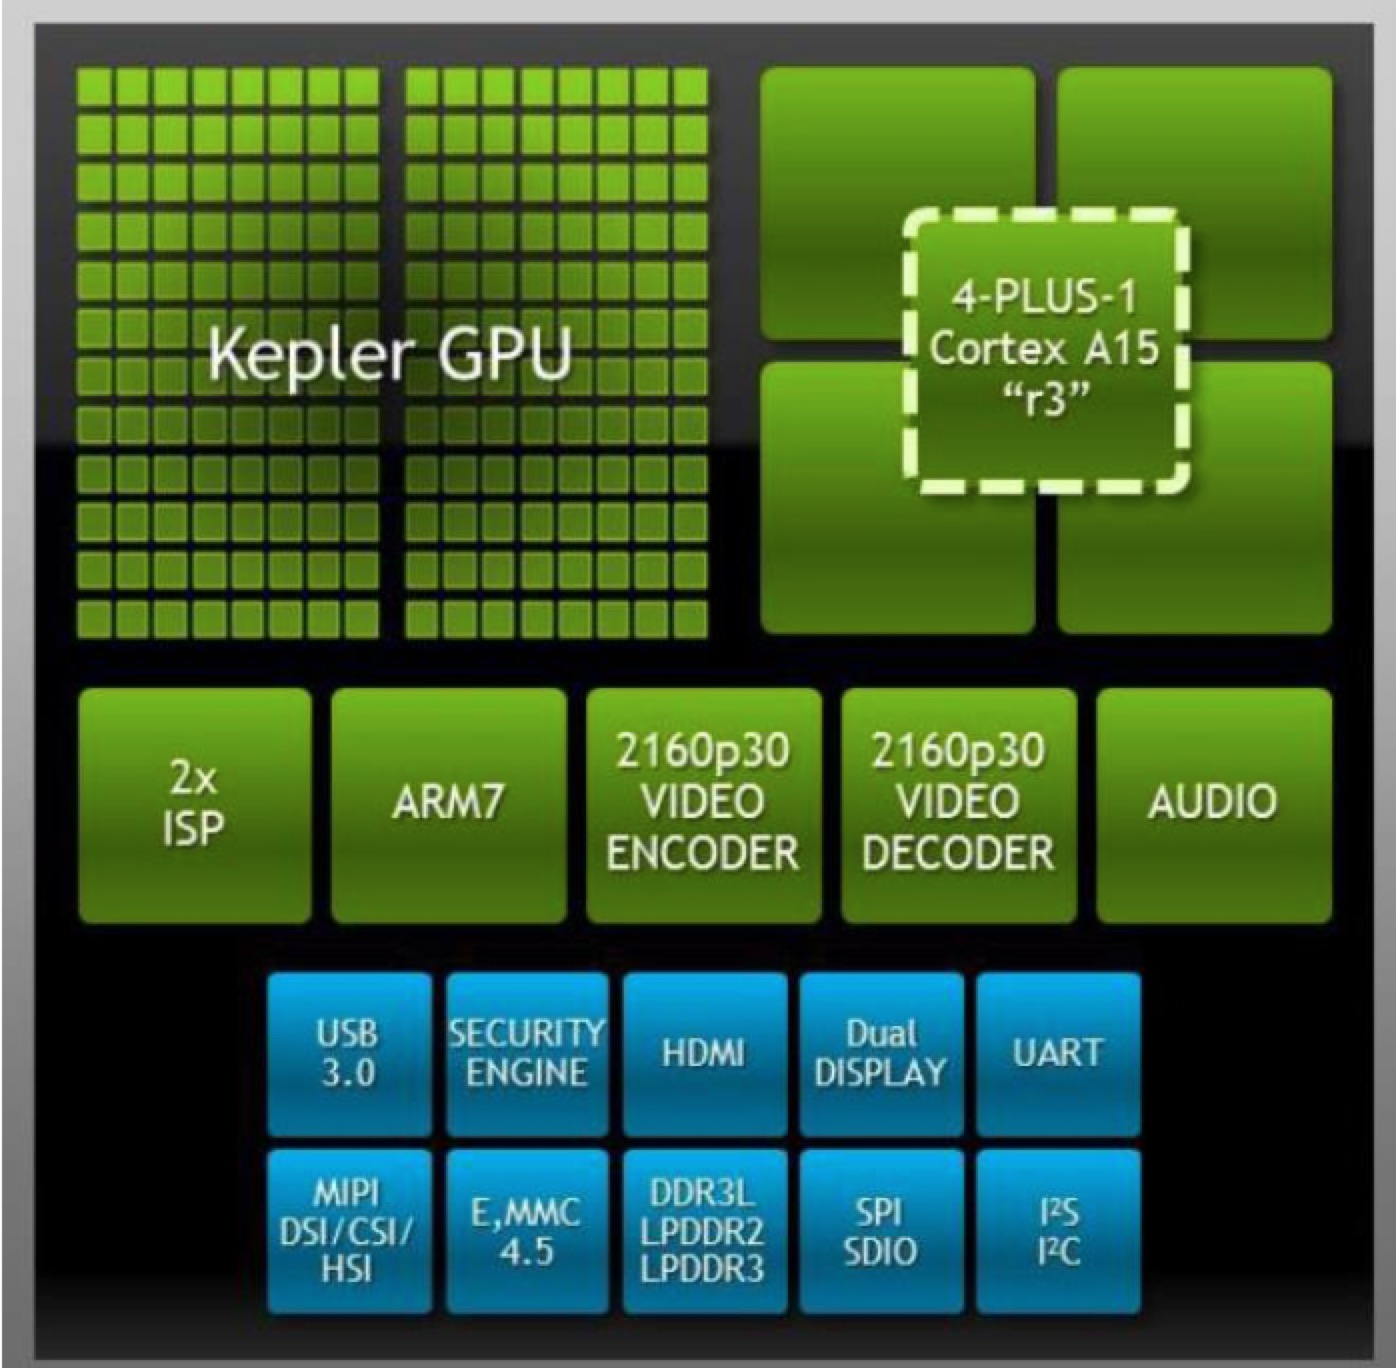
\includegraphics[width=0.5\textwidth]{tk1}
	\caption{Jetson TK1 硬件架构图}
	\label{fig:tk1}
\end{figure}

除了出色的硬件系统,该平台还拥有 OpenGL 4.4、CUDA VisionWorks 工具套 件等完备的支持软件,同时也包含有完整的开发套件和工具。此开发平台包含 1 个以并行运算平台和编程模型 CUDA 架构为基础的完整 C/C++工具套件,可让平 台比目前用于嵌入式系统的 FPGA、定制化 ASIC 和 DSP 处理器更容易进行程序 设计。

Jetson TK1 嵌入式平台具有广阔的应用前景,目前奥迪公司已经联手 NVIDA, 将利用 Jetson TK1 嵌入式平台开发自动驾驶系统。该平台将广泛应用于并行计算、 图像处理、数据分析等领域。

\subsection{CUDA编程模型}
CUDA是 NVIDIA 公司利用 GPU 平台进行通用并行计算的一种软件架构, CUDA 架构支持多种程序设计语言,同时 CUDA 架构可以充分发挥 GPU 的硬件优 势,从而大大提高程序运行速率。如今的 CPU 已经从单核发展到多核架构,每个处理核心都拥有容量较大的 Cache 以及复杂的控制逻辑和诸多优化电路。GPU 虽然拥有大量的核心,但是每 个核的设计工艺相对简单,只包含单纯的运算单元,没有复杂的逻辑判断硬件。在实际工程中也往往都采用 GPU 和 CPU 协同工作的模式,这种异构模式可 以发挥两种处理器的最大优势。这种模式下,CPU 用来完成内存的分配、数据的 拷贝及其他一些串行操作。GPU 用来完成数据的并行处理及其他一些并行的数学 运算。在这种协同模式下可以真正发挥两种处理器的强大功能,使程序运行速度 达到最佳。

\subsection{基于Jetson TK1 的深度学习目标检测算法}
Jetson TK1的GPU平台具有出色的并行计算的能力,而深度学习的前向计算过程是高度并行化的,特别适合用GPU做加速。本文采用CPU和GPU协同工作的模式将第 \ref{chap:2} 章中提出的基于深度学习的目标检测算法移植到Jetson TK1平台。本文采用caffe这种深度学习计算框架,将其移植到arm平台。caffe有众多的依赖库,例如opencv,boost,blans,libprotobuf,glog,gflags等。本文采用交叉编译的方式首先将这些依赖的库编译成静态文件,然后再将caffe编译成动态链接库,拷贝到arm上,完成运行时环境的搭建。caffe可以支持CUDA,因此直接将定义网络结构的protobuf文件输入给caffe便可直接进行计算。

由于TK1上GPU的现存容量有限,因此本文重新训练了一个小模型运行在其上。所谓小模型就是网络输入图片的分辨率被降低到$300\times500$,虽然如此,但本文提出的算法在此情况下的检测精度仍有68\%左右(在VOC 2007数据集上测试),能够使用大部分场景。且运行时间为300ms左右,为深度学习在嵌入式平台的应用提供了可能。